\documentclass[12pt, letterpaper]{article}
\usepackage{graphicx}
\usepackage{wrapfig}
\usepackage{indentfirst}
\usepackage[skip=10pt plus1pt, indent=40pt]{parskip}


\graphicspath{ {images/} }


\title{Comment calculer informatiquement une intégrale ?}
\author{Eliott Paquet}
\date{mai 2024}
\renewcommand*\contentsname{Sommaire}

\begin{document}
\maketitle

\tableofcontents
\newpage

\section{Introduction}
\subsection{Qu'est-ce qu'une intégrale ?}

Une intégrale correspond à l'air sous la courbe d'une fonction, c'est à dire, 
l'espace entre la courbe et l'axe des abscisses.
\par
\centering
Une intégrale se rédige de la manière suivante : 
\[ F(x)=\int_{a}^{b} x^2 \,dx \]
où a et b sont les bornes de notre intégrale.

\begin{wrapfigure}{r}{0.3\textwidth}
    \centering
    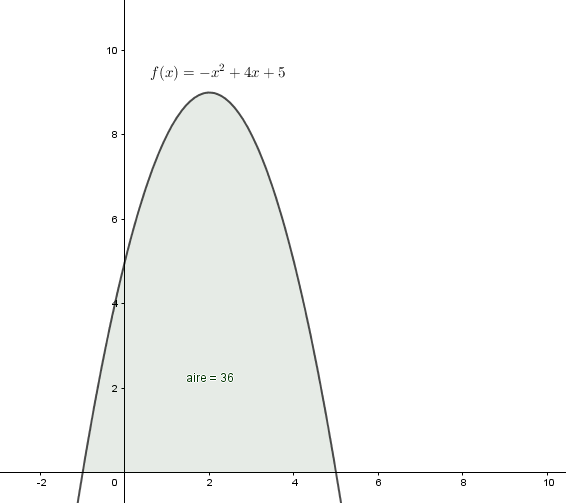
\includegraphics[width = 0.3\textwidth]{intégral.png}
    \caption{La courbe de $f(x)=-x^2 + 4x+5 $ }
\end{wrapfigure}

\raggedright
\linespread{100}
Dans le cas de la figure 1, l'intégral est :
\[ F(x) = \int_{{-1}}^{5} -x^2+4x+5 \,dx \]	
On pourrait traduire oralement cette expression par : "l'intégrale de -1 à 5 de \(-x^2 +4x+5\)"


\newpage
\subsection{Pourquoi avoir besoin d'une intégrale en informatique ?}
\section{Quels algorithmes ?}
\subsection{Somme de Riemann}
\subsection{Méthode de Monte-Carlo}
\subsection{Méthode de Simpson}
\listoffigures

\end{document}